\documentclass[reqno]{amsart}
\usepackage{amscd, amssymb, amsmath, amsthm}
\usepackage{amsfonts,enumerate}
\usepackage{latexsym,,txfonts}
\usepackage{graphics,graphicx,psfrag}
\usepackage{hyperref}
\usepackage[utf8]{inputenc}
\usepackage[T1]{fontenc}
\usepackage{textcomp}
\usepackage{babel}
\usepackage{tikz-cd}
\usepackage{biblatex}

\pdfsuppresswarningpagegroup=1

\newtheorem{theorem}{Theorem}[section]
\newtheorem{lemma}[theorem]{Lemma}
\newtheorem{proposition}[theorem]{Proposition}
\newtheorem{corollary}[theorem]{Corollary}
\newtheorem{conjecture}[theorem]{Conjecture}

\theoremstyle{definition}
\newtheorem{definition}[theorem]{Definition}
\newtheorem{example}[theorem]{Example}
\newtheorem{exercise}[theorem]{Exercise}
\newtheorem{problem}[theorem]{Problem}
\newtheorem{question}[theorem]{Question}

\theoremstyle{remark}
\newtheorem*{remark}{Remark}
\newtheorem*{note}{Note}
\newtheorem*{solution}{Solution}

\newcommand{\PSL}{\mathrm{PSL}}

\DeclareMathOperator{\Homeo}{Homeo}
\DeclareMathOperator{\ord}{ord}
\DeclareMathOperator{\Aut}{Aut}
\DeclareMathOperator{\lcm}{lcm}

\bibliography{refs}

\begin{document}



\section{Exercises and problems}

\begin{exercise}[Exercise 4.(b), week 3]
    Define one or two more charts to give $S$ the structure of a Riemann
        surface.
\end{exercise}

\begin{proof}
    For the last chart, I think something like the following should work:\\
    Take a small ball around each vertex of $P_m$ and intersect it
        with $P_m$. Let $V_i$ denote the open set at vertex $v_i$.
        Define a map $\psi_i \colon V_i \to \mathbb{C}$ by
        $\psi_i (z) = f_i \left( z - v_i \right) $, where
        $f_j \colon \mathbb{C} \to \mathbb{C}$ is given by
        \[
        f_j(re^{i \theta} ) = r e^{i \frac{2 \pi r_j}{n}} \left[ 
        e^{- i \left( \frac{(n-2 + 2j)\pi}{n} \right) } e^{i \theta}\right]^{\frac{2}{n-2}}
        \] 
        where $r_j$ is the smallest positive integer such that
        $r_j \left( \frac{m}{2}-1 \right) \equiv j \mod{m} $. Last part needs some modificaiton.
\end{proof}

\begin{exercise}[]\label{fuchsian-group-for-wiman-surfaces}
        Write down explicit $2 \times 2$ matrices that are generators for
        a Fuchsian group uniformizing the Wiman surfaces of Type I and Type
        II from the exercises from week 3.
    \end{exercise}

\begin{proof}
        We will construct the transformation as a composition of
        complex conjugation, followed by rotation and then inversion.\\
        Firstly, we wish to find the point of inversion: $\alpha = 
        a e^{i \theta}$.
        We have
        \begin{align*}
            \frac{L}{\sin \left( \frac{\pi}{2n} \right) }
            &= \frac{a}{\sin \left( \frac{(n+1) \pi}{2n} \right) }, \quad
            a^2 = 1 + L^2\\
            \implies a &= \sqrt{\frac{\sin^2 \left( \frac{(n+1)\pi}{2n} \right) }{
            \sin^2 \left( \frac{(n+1) \pi}{2n} \right) -
    \sin^2 \left( \frac{\pi}{2n} \right) }} \label{Omega}\tag{$\Omega$}
        \end{align*}
        And clearly $\theta = \frac{\pi}{2n}$. Now the inversion
        at $\alpha$ is given by
        \[
        \rho (z) = \frac{\alpha \overline{z} - 1}{\overline{z} - 
        \overline{\alpha}}
        \] 
        so all together we get the hyperbolic translation to be
        \[
        T(z) = \rho \left( e^{- \frac{(n-1)\pi i}{n}} \overline{z} \right) 
        = \frac{\alpha e^{\frac{(n-1) \pi i}{n}} z - 1}{
        e^{\frac{(n-1) \pi i}{n}} z - \overline{\alpha}}
        = \frac{a e^{\frac{\pi i}{2n}} e^{\frac{(n-1) \pi i}{n}} z - 1}{
        e^{\frac{(n-1) \pi i}{n} }z - a e^{- \frac{i \pi}{2n}}}
        = \frac{-a z - e^{\frac{i \pi}{2n}}}{-e^{\frac{- i \pi}{2n}} z-
        a}
        \] 
        Hence
        \[
        M(T) = 
        \begin{pmatrix} 
            a & e^{\frac{i \pi}{2n}}\\
            e^{- \frac{i \pi}{2n}} & a
        \end{pmatrix} 
        \] 
        Since $T_j = e^{\frac{(j-1) i \pi}{n}} T\left( 
        e^{- \frac{(j-1) i \pi}{n}} \right) $ we have
        \begin{align*}
            M(T_j) 
            &= \begin{pmatrix} e^{\frac{(j-1) i \pi}{n}} & 0 \\
            0 & 1\end{pmatrix} 
            \begin{pmatrix} a & e^{\frac{i \pi}{2n}}\\
            e^{- \frac{i \pi}{2n}} & a\end{pmatrix} 
                \begin{pmatrix} e^{- \frac{(j-1) i \pi}{n}} & 0\\
                0 & 1 \end{pmatrix} \\
            &= \begin{pmatrix} a & e^{\frac{(2j-1) i \pi}{2n}}\\
                e^{- \frac{(2j-1) i \pi}{2n}} & a
            \end{pmatrix} 
        \end{align*}
        where $a$ is given by \eqref{Omega}.
        So $\Gamma_n = \left< T_1, \ldots, T_n \right>$ is a Fuchsian group,
        and
        we have
        $W_{2n} \approx \mathbb{D} / \Gamma_n$.
    \end{proof}

    \begin{question}
        Check: consider why $\Gamma_n$ really is a Fuchsian group despite not having matrices in $\PSL(2,\mathbb{R})$.
    \end{question}


    \begin{exercise}
        Let $\mathcal{D}_k$ be the bipartification dessin of the map $M_k \colon R_k \hookrightarrow P_{2k} / \sim$.
        \begin{enumerate}
            \item Prove that
            $C_g^I \colon y^2 = x^{2g+1} -1, C_g^{II} \colon y^2 = x (x^{2g} -1)$ define Riemann surfaces isomorphic to
            $W_g^I, W_g^{II}$.
            \item 
            Determine rational functions $\beta_g^I$ and
            $\beta_g^{II}$ on
            $C_g^I$ and
            $C_g^{II}$ such that $(C_g^I, \beta_g^I)$ and
            $(C_g^{II}, \beta_g^{II})$ are Belyi pairs for $\mathcal{D}_{4g+2}$ and
            $\mathcal{D}_{4g}$, respectively.
        \end{enumerate}
    \end{exercise}

    \begin{proof}
        \textit{Idea:} If we can define two meromorphic functions
        $f,g \colon W_g^I \to \hat{\mathbb{C}}$ such that
        $\mathcal{M}(W_g^I) = \mathbb{C}(f,g)$ and such that
        $F(f,g) = 0$ for $F(X,Y) = Y^2 - X^{2g+1} +1$, then
        we are done by theorem 1.91.\\
        \linebreak
        \textit{Further remarks on this idea:}
        \begin{enumerate}
            \item This construction works for $P_4$ and
            $P_6$ since the polygons are equivalent to
            $\mathbb{C} / \Lambda$ for some lattice, and
            then corollary 2.12 gives the functions
            in the case of $P_4$ and example 4.21 gives
            the functions in the case of $P_6$. Can we
            generalize the construction of example 4.21?
            \item The naive direct approach would suggest
            not since to use the Weierstrass $\wp$ we
            need a lattice in $\mathbb{C} / \Lambda$ which
            gives a torus - however, we need higher genus
            surfaces.\\
            For this, we have the Poincaré series given
            in corollary 2.15. However, these are
            often hard to compute, so there's little hope here.
        \end{enumerate}
    \end{proof}

    \subsection{Project proposal exercises and problems}

Let $n = p^f$ be an odd prime power greater than $4$.
Let $h = \lfloor n/4 \rfloor$ - so in particular, in all of the following,
we are only interested in $h \geq 1$.
Let 
\[W = 
\begin{cases}
    W_{h}^I& \text{if }n\equiv 3 \pmod{4}\\
    W_h^{II}& \text{if } n\equiv 1 \pmod{4}
\end{cases}\]




    \begin{exercise}[Exercise 2]
        \begin{enumerate}
            \item Prove that $W$ is the underlying Riemann surface
            for the bipartification dessin $\mathcal{D}_k$ of
            $M_k$.
            \item Assuming problem A, prove that $S_{\mathfrak{p}}$
            is the underlying Riemann surface of a $K_n$-dessin.
        \end{enumerate}
    \end{exercise}

    \begin{proof}
        (1):\\
        \footnote{This proof contains technicalities which need to be checked.
        I imagine they work, but I'm not sure how to show it.}
        $W$ consists of two things: a topological structure which describes it as a topological $2$-manifold, i.e., a surface. And secondly, we add a structure to this surface which consists of
        a maximal atlas of certain charts - this is the complex structure on $W$ which we
        obtain from the Belyi map which we get from the dessin.\\
        So one way to look at this problem is that we want to show that the two structures on the topological surface coincide. What this means precisely, is that the charts from one structure is
        compatible with the charts from the other (since a maximal atlas contains all compatible charts).
        This would imply that the two structures are the same. One way of doing this also is to show that the Belyi map is holomorphic as a map
        $P_{n-1}/ \sim \to \hat{\mathbb{C}}$ with the Wiman surface structure.
        Now let's consider the charts
        arising from the Belyi map $\beta \colon P_n /\sim \to \hat{\mathbb{C}}$. 
        Without loss of generality, we can modify how the Belyi function maps the triangles onto
        the Riemann sphere. 

        \textit{Two approaches:}

        \begin{enumerate}
            \item Consider
        the hyperbolic plane as the Poincaré disk, and tessellate it
        according to the triangle group
        given in exercise 3.
        By \cite[Thm 3.7.(d)]{JW}, we can assume that $\beta$ maps
        a neighboring bicolored pair of triangles biholomorphically (considered
        as hyperbolic triangles in the Poincaré disk) onto
        $\hat{\mathbb{C}}$, where one triangle is mapped to the upper hemisphere
        and the other to the lower hemisphere, the boundary edges are mapped
        onto $\hat{\mathbb{R}}$ and the vertices are mapped to $0,1$ and $\infty$. This map induces
        a map on $\mathbb{D}/
        \left[\Delta, \Delta \right] 
        \approx W$.
        \item 
        We can again consider the
        hyperbolic plane as the Poincaré
        disk, but instead this time tessellate it purely using the
        side-pairing translations
        which give our Wiman surface.
        In this case, we are not dealing with a triangle group, but a subgroup (given in exercise 3). However, we can
        nonetheless proceed as in the
        proof of theorem 3.7.(d). 
        By the claims in the proof (which make use of a so called "stronger version of the Riemann mapping theorem", which I believe is the Schwarz-Christoffel mapping), we 
        can construct a function from
        a single monocolored triangle
        considered as a subset of $\mathbb{D}$ in its usual Riemann surface structure
        to $\hat{\mathbb{C}}$ such that
        the map is biholomorphic on the
        interior which it maps to
        the upper hemisphere, and such that it extends continuously onto
        the boundary and maps
        the vertices onto $0, 1$ and $\infty$. Now we can apply Schwarz's reflection principle to
        extend the map onto surrounding triangles. This process can be extended to define the function
        on all of $\mathbb{D}$, and this function becomes holomorphic outside the $\Delta$-orbits of
        the vertices of the triangle (by an application of Radó's theorem \cite{Radó}, I believe). At
        these points, we can continue
        $j$ by applying Riemann's removable singularity theorem (or just 
        \end{enumerate}
        

    

        By the remark in section~\ref{sec:algtop}, we have that aside from
        $\beta^{-1}\{0,1,\infty\}$, the Riemann surface structure is induced by
        $\beta$ being a covering map. On the face of the surface considered 
        under the face chart, $\beta$ simply
        maps a disk in the interior of $P_{n-1}/\sim$ to a disk in $\mathbb{C}$ holomorphically. Thus the transition map for the face map is just this map, which is hence holomorphic. All that's left to show is that the transition
        maps $\varphi_i$ are compatible too. But under the chart $\phi_i$, this
        will correspond to the union of two neighboring fundamental domain regions,
        and since the Belyi map is assumed to be $\Delta$-invariant, and there
        is a hyperbolic translation taking $U_i$ onto the neighboring fundamental domain, we have that the transition funciton will simply be a 2-fold ramified
        cover of $\hat{\mathbb{C}}$, and the restriction onto any open set
        on which it is injective will by assumption be biholomorphic. Since
        the charts for $\beta$ precisely guarantee that when we intersect the domains,
        the open subset of these fundamental domains will be such that $\beta$ is
        injective on them, we precisely find that the transition map is always biholomorphic for any induced by $\beta$. Thus we have shown that
        the charts $\phi_i$ and the face chart $\phi_F$ are compatible with the
        charts induced by $\beta$, so in particular the Riemann surface structures
        induced on $\Sigma -
        f^{-1}\{0,1,\infty\}$ are the same, so the result follows from proposition 
        \ref{RSiso}.
        \begin{figure}[http]
    \centering
    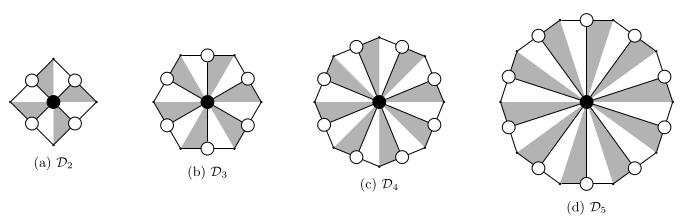
\includegraphics[width=1\linewidth]{bipartification-dessin-D_k.png}
    \caption{Four bipartification dessins and their
    associated triangulations}
    \label{fig:bipartification-dessin-D_k}
\end{figure}

        (2):

        We have the following commutative diagram:
        \begin{equation*}
            \begin{tikzcd}
                M_{\mathfrak{p}} \colon G_{\mathfrak{p}} \ar[r, hookrightarrow] \ar[d, "\pi_{\mathfrak{p}}"'] & S_{\mathfrak{p}} \ar[d, "\pi_{\mathfrak{p}}"] \ar[rd, dashed, "
                \tilde{\beta}"]  &\\
                M_k \colon R_k \ar[r, hookrightarrow] & P_{n-1}/\sim \ar[r, "\beta"'] & \hat{\mathbb{C}}
            \end{tikzcd}
        \end{equation*}
        We have one Belyi map
        $\beta$
        from part (a) of the exercise which
        we can lift to a Belyi map $\tilde{\beta}$ on
        $S_{\mathfrak{p}}$. 
        We claim that the
        induced structure by
        the covering map $\pi_{\mathfrak{p}}$
        is equivalent to the
        structure induced by the Belyi map
         $\tilde{\beta}$. The covering map
         $\beta$ has finite fiber over any point, and
         hence the composition of $\pi_{\mathfrak{p}}$
         and $\beta$ is a covering map away from
         ramification points, see \cite[Exercise 53.4]{Munkres}. Therefore, $\tilde{\beta}$
         induces a unique Riemann surface structure
         on $S_{\mathfrak{p}}$ making $\tilde{\beta}$
         holomorphic \ref{covering-induces-RS-structure}. But $\pi_{\mathfrak{p}}$ is
         holomorphic under a unique Riemann surface structure on $S_{\mathfrak{p}}$, and under this
         structure, the map $\beta \circ \pi_{\mathfrak{p}} = \tilde{\beta}$ is holomorphic as the composition of holomorphic functions. Thus, by uniqueness, the induced
         structures are the same. Now all that
         remains is to show that the underlying dessin
         for $\tilde{\beta}$ is a $K_n$ dessin. But
         this follows directly from
         problem A.(a), noting that the dessin
         for $\tilde{\beta}$ is
         $\tilde{\beta}^{-1}([0,1])$ which is
         precisely $G_{\mathfrak{p}}$ by construction
         which is a $K_n$ dessin. Thus we have
         the edges and the black vertices, and choosing
         the "midpoints" which are to be white vertices
         as the preimages of $1$ under $\tilde{\beta}$,
         we find that $\tilde{\beta}$ is a Belyi
         function arising from this bipartification dessin.
         This shows that the Riemann surface
         structure induced by the covering 
         $\pi_{\mathfrak{p}}$ is the underlying Riemann
         surface structure of a $K_n$-dessin.

\begin{remark}
    In fact, I think a little more can be shown
    using the Riemann surface structure
    of $P_{n-1} / \sim$ induced from
    $\beta$. Namely, the so called "midpoints" which
    we choose in the bipartification above
    to be $\tilde{\beta}^{-1}(1)$ should indeed correspond to the metric midpoint of the edges
    of $G_{\mathfrak{p}}$ under the
    metric induced by $\pi_{\mathfrak{p}}$.\\
     From the Riemann surface
         structure on $P_{n-1}/\sim$, we
         have a notion of lengths. This metric can be
         lifted locally to $S_{\mathfrak{p}}$ - i.e.,
          locally, $\pi_{\mathfrak{p}}$ becomes an
          isometry.
         Then taking the cover of
         $S_{\mathfrak{p}}$ of preimages
         of evenly covered open sets, we can
         for any two points $x$ and $y$ in $S_{\mathfrak{p}}$ take the distance between
         them to be the infimum of distances of
         paths running between $x$ and $y$ where
         this distance is calculated by subdividing
         the path into a finite number of line segments (using compactness) contained in a connected
         component of the preimage of an evenly covered set on which we have the inherited metric. It is then clear that
         the length of such a path is the same - i.e.,
         the length of a path in
         $P_{n-1}/\sim$ is the same as the
         length of its lift - and hence midpoints (understood in its geometric notion using a metric) are well-defined and preserved
         under the lift. So since the white vertices
         in $P_{n-1}/\sim$ were, I believe, chosen
         to be the metric midpoints, the white
         vertices lift to midpoints on the edges
         above too.
         Thus we have that $\tilde{\beta}$ indeed
         corresponds to the Belyi map induced by
         the bipartification considering
         midpoints as geometric midpoints.
\end{remark}
         
    \end{proof}
    
By the Uniformization theorem, $W$ is isomorphic to
$\mathbb{U}/ \Gamma$, where $\mathbb{U}$ is either the Riemann
sphere $\mathbb{P}^1 (\mathbb{C})$, the complex plane $\mathbb{C}$,
or the unit disk $\mathbb{D}$, depending on whether
$h = 0$, $h=1$ or $h\geq 2$, respectively, and
$\Gamma \leq \Aut (\mathbb{U})$. Fix an isomorphism
$\Gamma \cong \pi_1 (P_{n-1}/\sim)$. Write $\Gamma_{\mathfrak{p}}$ for the subgroup of $\Gamma$ corresponding
to $H_{\mathfrak{p}} \trianglelefteq \pi_1 (P_{n-1}/\sim)$.

We have 
    \[
    \Delta (l,m,n) =
    \langle x_1, x_2 \mid 
    x_1^l = x_2^m = (x_1 x_2)^{n} = 1
    \rangle.
    \]
    By definition, the commutator is
    the kernel of the inclusion map
    of $\Delta$ into its abelianization, i.e.,
    the following sequence is exact:
    \[
    \left[ \Delta, \Delta \right] \hookrightarrow
    \Delta \to \Delta^{ab}
    \]

    We have from \cite[p~105]{Albar-Al-Hamdan} that 
   \[
    \Delta^{ab}
    \approx Z_{d_1} \times Z_{d_2}\]
where
\[d_1 = \gcd(2,4h,4h) = 2, \quad
\text{and} \quad d_2 = \frac{\gcd(8h, 8h, 16h^2)}
{d_1}
= 4h\]
so $\Delta^{ab}
    \approx Z_2 \times Z_{4h}$ when
    $\Delta = \Delta (2,4h, 4h)$, and
    when $\Delta = \Delta (2,2h+1,4h+2)$, we
    get $d_1 = 1$ and $d_2 = 4h+2$, so
    $\Delta^{ab} \approx Z_{4h+2}$.

\begin{exercise}[Exercise 3]
    Let $\Delta$ be the ordinary triangle group
    \[ \Delta = 
    \begin{cases}
        \Delta (2, 2h+1, 4h+2),& \text{if } n \equiv 3 \pmod{4}\\
        \Delta (2,4h,4h),& \text{if } n\equiv 1  \pmod{4}
    \end{cases}
    \]
      \begin{enumerate}
        \item \textit{Guess for problem statement:} 
        For $n \equiv 3 \pmod{4}$,
    let $\Gamma = 
        \left[\Delta, \Delta \right]$, and for $n \equiv
        1 \pmod{4}$, let $\Gamma$ be the kernel of
        the abelianization map composed with the projection onto the $Z_{4h}$ factor of $\Delta^{ab} \approx Z_2 \times
        Z_{4h}$. Prove that $\Gamma$ uniformizes 
        $W$, i.e., $W$ is isomorphic to
        $\mathbb{U}/ \Gamma$.
        \item Prove that the quotient
        projection
        $\mathbb{U}/ \Gamma_{\mathfrak{p}} \to
        \mathbb{U}/ \Delta$ is a 
        Belyi function for a
        $K_n$-dessin.
    \end{enumerate}
\end{exercise}

\begin{proof}
    (1)

    We know by Kulkarni's theorem that for $h >3$,
    $W \approx \mathbb{U}/ \left[\Delta, \Delta \right]$ if and only if
    $\Aut (\mathbb{U}/ \left[\Delta, \Delta \right]) $ contains a cyclic subgroup of
    order $4h+2$ (or $4h$ depending on what the type of the Wiman surface is) and $\mathbb{U}/ \left[\Delta, \Delta \right]$
    has genus $h$.\\
    \linebreak

    \textit{Case: $h > 3$}

There is a paper by Harvey \cite{Harvey} which might be useful for the following two parts.\\
\linebreak






\textit{Showing it has a cyclic subgroup of order $4h+2$
or $4h$:}\\
\linebreak

We know \cite[Prop. 2.35]{Girondo-Gonzalez-Diez} that 

\begin{align*}
\Aut( \mathbb{H} / \Gamma) 
&\approx
N(\Gamma)/ \Gamma.
\end{align*}

We have by the first isomorphism theorem, we know that
\[\Delta / \Gamma \approx Z_{4h}.\]
And since $\Gamma$ is the kernel of a homomorphism from
$\Delta$ into some group, $\Gamma$ is normal in $\Delta$, so
$\Delta \leq N(\Gamma)$.
Hence

\[\Aut (\mathbb{H}/\Gamma) \approx
N(\Gamma) / \Gamma \geq \Delta / \Gamma \approx 
\begin{cases}
    Z_{4h+2},& \text{if } n \equiv 3 \pmod{4}\\
    Z_{4h},& \text{if } n \equiv 1 \pmod{4}
\end{cases}
\]


\textit{Showing that the genus is $h$:}\\

Let $g$ denote the genus of $\mathbb{H}/\Gamma$. By definition, our constructing maps
$\Delta \to Z_{4h}$ and $Z_{4h+2}$ are
surface-kernel maps as the kernel is a subgroup
of a triangle group and thus has no periods and is therefore a Fuchsian surface group. 

Therefore, we know that the orders of each
generator $x_i$ is still $m_i$ in $Z_{4h+2}$ or
$Z_{4h}$. So since these groups act on
$\mathbb{H}/ \Gamma$ by the first part of the problem, we can apply the Riemann-Hurwitz theorem, in the form provided by Harvey, \eqref{Riemann-Hurwitz-Harvey}, giving us for $n \equiv 3 \pmod{4}$,

\[\frac{2 (g-1)}{4h+2} = 
-2 + 3 - \frac{1}{2} - \frac{1}{2h+1} - \frac{1}{4h+2}
= 1 - \frac{h+2}{2h+1}\]
(note that $\gamma$ is clearly $0$ visually, but this needs a better argument) which gives
\[g = 1 + \frac{1}{2} \left( 2h-2 \right)
= h \]
and in the case of $n \equiv 1 \pmod{4}$,
we get
\[\frac{2(g-1)}{4h}
= 1 - \frac{1}{2} - \frac{1}{4h} - \frac{1}{4h}\]
which gives
\[g = 1 + \frac{1}{2} 2(h-1) = h.\]


So the genus of $\mathbb{H}/\Gamma$ is $h$
as required. Now Kulkarni's theorem guarantees that $\mathbb{H}/\Gamma \approx W$.\\
\linebreak







(2): 
\textit{Idea:} Use corollary \ref{fuchsian-triangle-induce-belyi}

\begin{equation*}
            \begin{tikzcd}
                H_{\mathfrak{p}} 
                \ar[d, dash, "\approx"]\ar[r,
                hookrightarrow] & \pi_1 (P_{n-1}/\sim) \approx
                \left[\Delta, \Delta \right]\ar[d, dash, "\approx"]
                \ar[r,hookrightarrow]&
                \Delta
                \\
                \Gamma_{\mathfrak{p}} 
                \ar[r, hookrightarrow]&
                \Gamma
            \end{tikzcd}
        \end{equation*}

        To show that the map is
        a Belyi map, we must show that $\Gamma_{\mathfrak{p}}$ is a Fuchsian group and that it is
        contained in $\Delta$.

        For the containment, we have by
        construction that we can think
        of this as the subgroup
        $H_{\mathfrak{p}}$ which
        is contained in
        $\pi_1 (P_{n-1}/\sim) 
        \approx \left[ \Delta, \Delta
        \right] \leq \Delta$.

        Now for the Fuchsian part, 
        this follows from the fact
        that subgroups of Fuchsian groups
        are also Fuchsian groups, and
        $\Delta$ is a Fuchsian group.

        It only remains
        to show that the preimage
        of the interval
        $\left[ 0,1 \right]
        \subset \mathbb{C}\mathbb{P}^1
        \approx \mathbb{U}/ \Delta$
        is a $K_n$-dessin.

 
    
    








    
\end{proof}



\newpage


\subsection{Random stuff we might need}
\begin{enumerate}
        \item We have checked that for the case of $P_6$ for example,
        we indeed get that the commutator elements like $x_1 x_2 x_1^{-1}
        x_2^{-1}$ correspond to translations in the plane which precisely
        match the side pairing translations used to construct the Wiman surface.
        It thus remains to check that all elements in the commutator
        subgroup correspond to compositions of these translations. 
        See \ref{fig:P_6-commutators}.
        \begin{figure}[http]
            \centering
            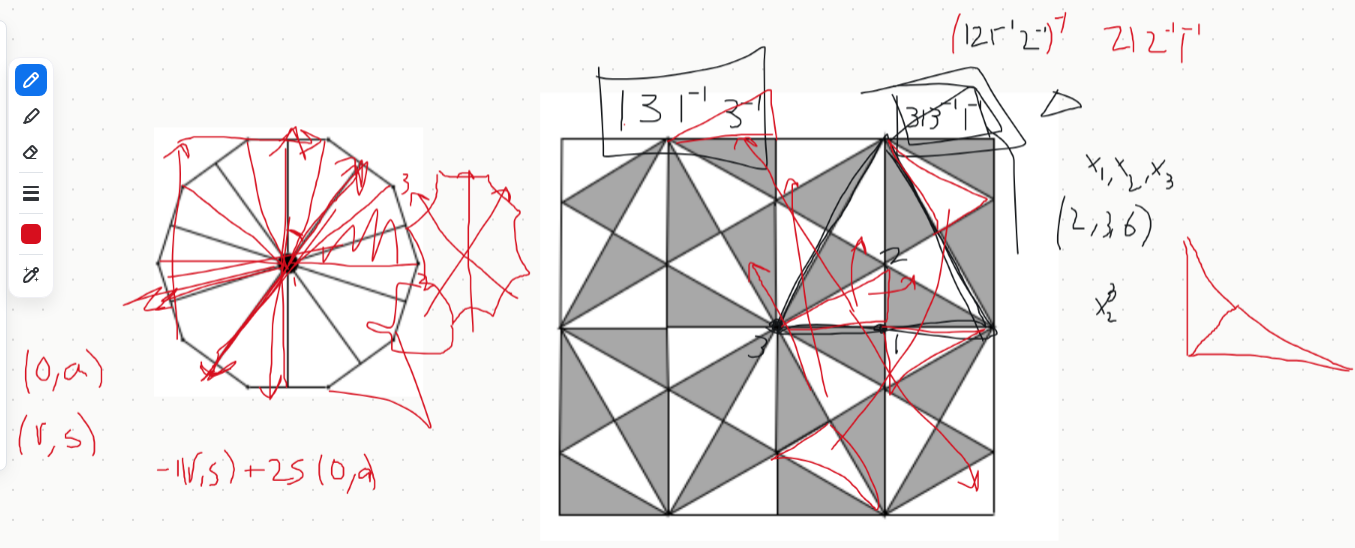
\includegraphics[width=1.2\linewidth]{P_6-commutators.png}
            \caption{Group meeting on 07/08/24. Sketch of how one can trace the image of the triangle
            in the tessellation}
            \label{fig:P_6-commutators}
        \end{figure}
        \item The question then becomes whether we can generalize this process
        to $h \geq 2$ where instead the tessellation becomes of the hyperbolic
        plane. Intuitively things should work out the same, however, there
        will be more side-pairings to check, and precisely how to find the
        corresponding commutators, we don't know yet. 
        \item A thing to note is that for $h \geq 2$, we have an explicit
        description of the uniformizing group (aka surface group) for
        the Wiman surface, given in exercise 
        \ref{fuchsian-group-for-wiman-surfaces}. So one way to rephrase the
        problem is: find an isomorphism $\left[\Delta, \Delta \right] 
        \approx \Gamma_n$ for $\Gamma_n$ given as in the exercise. 
        \item Another approach is to find the formulas for the hyperbolic
        rotations around each of the vertices. This shouldn't be particularly
        hard, and it would give an explicit description of $\Delta$ in
        terms of matrices. Perhaps it would be doable to find the commutator
        group of this group of matrices?
        \item The figures under the classification section might be of use for visualization: 
        \url{https://en.wikipedia.org/wiki/Triangle_group}
    \end{enumerate}


    \[
    \begin{tikzcd}
        \mathbb{H} \ar[d, "\pi"']
        \ar[dr, "j"] & \\
        P_{n-1}/\sim \ar[r, dashed, "\beta"'] & \mathbb{C}\mathbb{P}^1
    \end{tikzcd}
    \]

\section{Notes and background}

\subsection{Algebraic Topology}



\begin{proposition}
    If $p \colon X \to Y$ is a covering space with $X$ path-connected and
    $Y$ simply-connected, then $p$ is a homeomorphism.
\end{proposition} 

\begin{corollary}
    Suppose $X$ is a connected Riemann surface and $Y$ is a simply connected
    Riemann surface. If $f \colon 
    X \to Y$ is an unramified morphism then it is an isomorphism.
\end{corollary}


\begin{remark}\label{sec:algtop}
    If $p \colon E \to X$ is a covering map between
    surfaces, and $X$ has a Riemann surface structure, then
    $E$ inherits a unique Riemann surface structure such that
    $p$ is holomorphic. The structure on $E$ is given by
    charts $(U_i, \phi_j \circ p)$ where
    $(V_j, \phi_j)$ is a chart on $X$ and
    $p (U_i)= V_j$ is an evenly covered (aka. well-covered) neighborhood.\\
    So essentially, we just define charts on the patches that
    are homeomorphic to evenly covered patches downstairs.
\end{remark}


\subsection{Complex Analysis}
Here are a few of the important things to keep in mind.

\begin{remark}
    A holomorphic map is conformal at any point where its derivative is non-vanishing. 
\end{remark}

\begin{theorem}
    Suppose $f \colon G \to \mathbb{C}$ is
    holomorphic in an open set
    $G \subset \mathbb{C}$ and that
    $f$ is bijective. Then
    $f(G)$ is open in $\mathbb{C}$ and
    the inverse function
    $f^{-1} \colon f(G) \to G$ is
    holomorphic with
    \[
    (f^{-1})' = \frac{1}{f' \circ
    f^{-1}}
    \]
    In particular,
    $f'(z) \neq 0$ for all
    $z \in G$.
\end{theorem}

\begin{remark}
    It is also a topological result that
    if only $f \colon G \to \mathbb{C}$
    is bijective and continuous, then
    $f(G)$ is open in $\mathbb{C}$ and
    $f^{-1} \colon f(G) \to G$ is
    continuous.
\end{remark}

\begin{theorem}[Riemann's removable singularity theorem]\label{removable-singularity-thb}
    Assume that $f \in \mathcal{H}
    (K'(a,r))$ is bounded in
    $K'(a,r)$. Then $f$ has a removable
    singularity at $a$.
\end{theorem}

\begin{theorem}[Riemann's mapping theorem]\label{Riemann-mapping-thm}
    Let $G$ be a simply connected domain different
    from $\mathbb{C}$. Then there exists a 
    biholomorphism $\phi \colon G \to K(0,1)$.
\end{theorem}



\subsubsection{Useful things to know:}
\begin{itemize}
    \item Different types of singularities:
    removable, poles and essential, and their correspondence with the Laurent
    expansion of a holomorphic function.
\end{itemize}


\subsection{Riemann surfaces}
\begin{center}
    Most of the things laid out below are arguments that are swept under the rug in certain parts
of section 3 on Belyi functions in Girondo and Gonzalez-Diez's book. They can function as
supplying more detail. Some parts are also used
in the exercises and problems above.
\end{center}



\begin{lemma}\label{covering-induces-RS-structure}
    Let $Y$ be a compact Riemann surface,
    $\Sigma \subset Y$ a finite subset, 
    $Y^* = Y - \Sigma$. Assume that
    $f^* \colon X^* \to Y^*$ is an
    unramified holomorphic covering
    of finite degree. Then there
    exists a unique compact Riemann
    surface $X \supset X^*$ such that
    $f^*$ extends to a unique morphism
    $f \colon X \to Y$.\\
    Moreover, $X - X^*$ is a finite
    set.
\end{lemma}

\begin{proposition}\label{RSiso}
    Let $X_1$ (resp. $X_2$) be a compact
    Riemann surface, and 
    $\Sigma_1 \subset X_1$ (resp. 
    $\Sigma_2 \subset X_2$) be a finite set. Assume that $X_1^* =
    X_1 - \Sigma_1$ and
    $X_2^* = X_2 - \Sigma_2$ are isomorphic. Then $X_1$ and
    $X_2$ must be isomorphic too.
\end{proposition}

\begin{lemma}
    If $\Gamma$ is a triangle group, then by proposition 2.21, $\mathbb{D}/\Gamma$ is a Riemann
    surface, which we can see must have genus $0$. Thus
    $\mathbb{D} / \Gamma \approx \hat{\mathbb{C}} - \Sigma$ where
    $\left| \Sigma \right| \in \{0, 1,2,3\}$.
\end{lemma}

\begin{remark}\label{order of point}
    For some Fuchsian group $\Gamma$ which, wlog. we can assume acts on $\mathbb{D}$ instead of 
    $\mathbb{H}$, we have that $\ord_z \pi = \left| I(z) \right|$, where
    $\pi \colon \mathbb{D} \to \mathbb{D} / \Gamma$ is the quotient map which is holomorphic.
\end{remark}

\begin{corollary}\label{fuchsian-triangle-induce-belyi}
    As a result of the above remark and lemma, we have that if $K$ is a Fuchsian group
contained in some triangle group $\Gamma = \Gamma_{n,m,l}$ with
$n,m,l \in \mathbb{Z}$, then the quotient map  $\mathbb{D}/K \to
\mathbb{D}/\Gamma$ is a Belyi function.
\end{corollary}


\subsubsection{Endowing the topological surface of a dessin with a Riemann surface structure}
To some dessin $(X, \mathcal{D})$, we
obtain a triangle decomposition
$\mathcal{T} = \mathcal{T}(\mathcal{D})$.\\
To each triangle
$T_j^{\pm}$, we construct a homeomorphism
$f_j^{\pm} \colon T_j^{\pm}
\to \overline{\mathbb{H}}^+ =
\mathbb{H} \cup \mathbb{R}\cup 
\{ \infty\}$
 satisfying
 \[
f_j^{\pm} \colon
\begin{cases}
    \partial T_j^{\pm} &\longrightarrow  \mathbb{R}\cup
    \{\infty\}\\
    \circ &\longrightarrow  0\\
    \bullet &\longrightarrow 1\\
    \times &\longrightarrow  \infty
\end{cases}
 \]

Then we glue together the collection
of homeomorphisms $\{f_j^{\pm}\}$
to obtain a continuous function
$f_{\mathcal{T}(\mathcal{D})} \colon X
\to \hat{\mathbb{C}}$ whose restriction
$f_{\mathcal{T}(\mathcal{D})} \colon
X^* = X - f_{\mathcal{T}(\mathcal{D})}^{-1} \{0,1,\infty\} \to
\hat{\mathbb{C}}- \{0,1,\infty\}$ is
a covering map. This gives
$X^*$ a unique Riemann surface structure such that
$f_{\mathcal{T}(\mathcal{D})}$ is holomorphic on $X^*$ (see section 1.2.5 in Girondo and Gonzalez-Diez). Then we can extend uniquely to
a holomorphic function on
$X$ by Lemma~\ref{covering-induces-RS-structure}.
Then $X$ inherits a unique
Riemann surface structure with which $X$ is denoted by
$S_{\mathcal{T}(\mathcal{D})}$.

\subsubsection{Function fields}
Let $S$ be a compact
Riemann surface.
\begin{proposition}
    Suppose
    $f \in \mathcal{M}(S)$ has degree
    $n$. Then the extension
    $\mathcal{M}(S) /
    \mathbb{C}(f)$
    has degree $n$.
\end{proposition}

\begin{corollary}
    By the primitive
    element theorem, we thus have that
    $\mathcal{M}(S)
    = \mathbb{C}(f,g)
    $ for some
    meromorphic functions $f,g$
    where $g$ is
    not a root in
    $\mathbb{C}(f)$.
\end{corollary}

\begin{theorem}
    Let $\mathcal{M}(S) = \mathbb{C}(f,h)$, and
    let $F (X,Y)$ be
    an irreducible polynomial such that $F(f,h) 
    \equiv 0$. Then
    the map $\Phi \colon S \to S_F$ given by
    $P \mapsto (f(P),
    h(P))$ defines an isomorphism.
\end{theorem}

Here the existence of
$F$ is just because
of the nature of
how we define degrees
of finite extensions
and the above
proposition.

\begin{definition}
    A function field of $n$ variables over a field $k$ is a finite field extension of the field $k(x_1, \ldots, x_n)$ of rational functions in $n$ variables over $k$.
\end{definition}

\begin{proposition}
    The functor
    $\mathcal{M}(\cdot)$ which sends Riemann surfaces to their
    function fields
    and maps between Riemann surfaces to
    the induces maps,
    $f \mapsto f^*$ where $f^*(g) = 
    g \circ f$,
    establishes a duality (contravariant equivalence) between the categories of
    Riemann surfaces and function fields in one variable.
\end{proposition}

\subsubsection{Wiman surfaces}
\begin{theorem}[Wiman]
    The order of any automorphism of a compact
    connected Riemann surface of genus $g$ is at
    most $4g+2$.
\end{theorem}

\begin{theorem}[Kulkarni]
    For each $g \geq 2$, there is a unique
    Wiamn surface of type I. For $g \geq 3$, there is a unique Wiman surface of type II.
    For $g = 3$, there are two Wiman surfaces of type II, up to isomorphism.
\end{theorem}

\subsection{Harvey's paper}

\begin{question}[The central question:]
    What is the minimum genus of a surface for which a given finite
    group $G$ is a group of automorphisms?
\end{question}

\begin{definition}\label{fuchsian-group-presentation}
    If a Fuchsian group $\Gamma$ has compact orbit space,
    its is known to have the following structure:
    \[
    \langle x_1, x_2, \ldots x_n, a_1, b_1, a_2, b_2 ,\ldots,
    a_{\gamma} , b_{\gamma} \mid 
    x_1^{m_1} = x_2^{m_2} = \ldots = x_n^{m_n} =
    x_1 \cdots x_n \Pi_{i=1}^{\gamma} \left[a_i, b_i \right] =1 \rangle,
    \]
    where, if $\gamma = 0$, the last relation
    is considered as $x_1 \cdots x_n = 1$.
    Following Macbeath's nomenclature, the integers
    $m_1, \ldots, m_n$ (all different from $1$) are called the
    \textit{periods} of the group $\Gamma$, and
    $\gamma$ is called the \textit{orbit genus}. If there
    are no periods, the group is called a Fuchsian \textit{surface group}.\\
    For brevity, we sometimes refer to a Fuchsian group with
    the above presentation by the name
    $(m_1, m_2, \ldots, m_n ; \gamma)$\textit{-group}.
\end{definition}

\begin{remark}
    Note in particular, that the
    $(m_1, m_2, m_3;0)$-group is
    precisely the (ordinary triangle group) von Dyck group $\Delta(m_1, m_2,m_3)$.
\end{remark}

\begin{definition}
    Each Fuchsian group $\Gamma$ has
    a fundamental region $F_{\Gamma}$
    in the upper half plane
    $\mathbb{H}$; and a non-Euclidean
    measure of $F_{\Gamma}$, $\mu (F_{\Gamma})$, given by
    \[\mu (F_{\Gamma}) =
    2 \pi \left[ 2 (\gamma -1)
    + \sum_{i=1}^n \left(1-\frac{1}{m_i}
    \right) \right] \]
    where $\Gamma$ is the
    $(m_1, \ldots, m_n; \gamma)$-group.
\end{definition}

\begin{question}
    Harvey claims that groups
    such as $\Delta(2,3,4)$ and
    $\Delta(2,4,4)$ do not
    define Fuchsian groups with
    compact orbit space. How does this make sense? Aren't the orbit spaces the sphere?
    Is it because we are talking
    about how these groups act
    on the hyperbolic plane, not 
    the complex plane?
\end{question}

\begin{theorem}
    Any compact Riemann surface
    $S$ of genus $g \geq 2$
    is representable as an orbit
    space $D/K$ where $K$,
    a Fuchsian surface group with orbit genus $g$,
    is the fundamental group of
    $S$, and $\mathbb{H}$, the upper half plane, is the universal covering space of $S$.
\end{theorem}

\begin{remark}
    This makes sense
    as we have an explicit
    description of
    $\pi_1(\Sigma_n)$ for
    all $n$ which coincides
    with the structure of a surface group of
    orbit genus $n$ given
    in the definition above.
\end{remark}

\begin{theorem}
    A finite group $G$ acts
    as a group of automorphisms
    of some compact Riemann surface
    of genus $g \geq 2$, if
    and only if $G$ is isomorphic to the \textit{factor group}
    $\Gamma /K$, where
    $\Gamma$ is a Fuchsian group with compact orbit space, and $K$ is a Fuchsian group with orbit genus $g$.
\end{theorem}

\begin{theorem}[Hurwitz]
    The number of automorphisms of a compact Riemann surface of genus $g \geq 2$ never exceeds
    $84 (g-1)$.
\end{theorem}



\subsubsection{Surface-kernel homomorphisms and automorphism
groups}

\begin{definition}
    A surjective homomorphism 
    $\Gamma \to G$, where
    $\Gamma$ is a Fuchsian group and $G$ is finite, such that the kernel is a Fuchsian surface group $K$,
    is termed \textit{surface-kernel}, and the corresponding finite group
    $\Gamma / K \approx G$ is
    a \textit{surface-kernel factor group}.
\end{definition}

For such a group we have
$\left| G \right| =
\frac{\mu (F_K)}{\mu(F_{\Gamma})}$,
where $F_K, F_{\Gamma}$ are
fundamental regions for
$K$ and $\Gamma$, respectively.
This gives us
the following Riemann-Hurzwitz
identity (compare to its form
in \cite[Lemma~2.39]{Girondo-Gonzalez-Diez}):
\[
\frac{2(g-1)}{\left|G\right|}
= 2 (\gamma -1) + 
\sum_{i=1}^n \left(1-
\frac{1}{m_i} \right) \tag{$\zeta$}\label{Riemann-Hurwitz-Harvey}
\]
for admissable $\Gamma$ with presentation~\ref{fuchsian-group-presentation}.


\begin{theorem}[Bundgaard, Nielsen and Fox]
    Every Fuchsian group $\Gamma$ possesses as surface group $K$ as a normal subgroup of finite index.
\end{theorem}

\begin{theorem}
    A homomorphism 
    $\phi$ form a Fuchsian group $\Gamma$ onto
    a finite group $G$ is surface-kernel if and only if it preserves the periods of $\Gamma$,
    i.e., for every periodic generator
    $x_i$, of order
    $m_i$, $\phi (x_i)$ has
    order $m_i$.
\end{theorem}

\begin{proof}
    If the homomorphism is surface-kernel, then
    suppose $x_i$ has
    order $m_i$. Then
    $1 = \phi(x_i)^{m_i}$,
    so the order divides $m_i$. If its order was
    strictly less, then
    $x_i^r$ would be in $K$
    for some $r < m_i$. But
    $K$ is a subgroup of 
    $\Gamma$ which
    is a surface group, so
    it contains no period
    elements. Hence
    it cannot contain $x_i^r$.\\
    \linebreak
    The other direction is given in the text with a certain "well-established result". 
\end{proof}

\begin{theorem}
    Let $\Gamma$ have presentation ~\ref{fuchsian-group-presentation}, and
    let $M = 
    \lcm (m_1, \ldots, m_n)$.
    There is a surface-kernel
    homomorphism
    $\phi \colon \Gamma
    \to Z_N$ if and only
    if the following conditions are satisfied:
    \begin{enumerate}
        \item 
        $\lcm(m_1, \ldots,
        \hat{m_i}, \ldots
        , m_n) = M$ for
        all $i$, where
        $\hat{m_i}$ denotes
        the omission of $m_i$;
        \item $M$ divides
        $N$, and if
        $\gamma = 0$, 
        $M = N$;
        \item $n\neq 1$, and
        , if $\gamma = 0$,
        $n \geq 3$;
        \item if $2 \mid M$,
        the number of periods divisible by the maximum power of $2$ dividing $M$ is even.
    \end{enumerate}
\end{theorem}


\begin{theorem}
    Given a cyclic group $Z_N$ ($N \neq 2,3,4$ or $6$), the minimum value of $g$ corresponds to a surface-kernel homomorphism from a Fuchsian triangle group onto $Z_N$.
\end{theorem} 

\begin{theorem}
    The minimum genus $g$ of a surface which admits an automorphism of order $N= p_1^{r_1} \ldots p_k^{r_k}$ is given by
    \begin{enumerate}
        \item $g = 
        \max \left\{ 2, \frac{p_1 - 1}{2} \frac{N}{p_1} \right\}$, \quad if $r_1 > 1$ or
        $N$ is prime,
        \item $g = 
        \max \left\{
        2, \frac{p_1 - 1}{2} \left(\frac{N}{p_1} - 1  \right)
        \right\},$ \quad
        if $r_1 = 1$.
    \end{enumerate}
\end{theorem}


















\newpage
\printbibliography

\end{document}
